% Options for packages loaded elsewhere
\PassOptionsToPackage{unicode}{hyperref}
\PassOptionsToPackage{hyphens}{url}
\documentclass[
]{article}
\usepackage{xcolor}
\usepackage{amsmath,amssymb}
\setcounter{secnumdepth}{-\maxdimen} % remove section numbering
\usepackage{iftex}
\ifPDFTeX
  \usepackage[T1]{fontenc}
  \usepackage[utf8]{inputenc}
  \usepackage{textcomp} % provide euro and other symbols
\else % if luatex or xetex
  \usepackage{unicode-math} % this also loads fontspec
  \defaultfontfeatures{Scale=MatchLowercase}
  \defaultfontfeatures[\rmfamily]{Ligatures=TeX,Scale=1}
\fi
\usepackage{lmodern}
\ifPDFTeX\else
  % xetex/luatex font selection
\fi
% Use upquote if available, for straight quotes in verbatim environments
\IfFileExists{upquote.sty}{\usepackage{upquote}}{}
\IfFileExists{microtype.sty}{% use microtype if available
  \usepackage[]{microtype}
  \UseMicrotypeSet[protrusion]{basicmath} % disable protrusion for tt fonts
}{}
\makeatletter
\@ifundefined{KOMAClassName}{% if non-KOMA class
  \IfFileExists{parskip.sty}{%
    \usepackage{parskip}
  }{% else
    \setlength{\parindent}{0pt}
    \setlength{\parskip}{6pt plus 2pt minus 1pt}}
}{% if KOMA class
  \KOMAoptions{parskip=half}}
\makeatother
\usepackage{graphicx}
\makeatletter
\newsavebox\pandoc@box
\newcommand*\pandocbounded[1]{% scales image to fit in text height/width
  \sbox\pandoc@box{#1}%
  \Gscale@div\@tempa{\textheight}{\dimexpr\ht\pandoc@box+\dp\pandoc@box\relax}%
  \Gscale@div\@tempb{\linewidth}{\wd\pandoc@box}%
  \ifdim\@tempb\p@<\@tempa\p@\let\@tempa\@tempb\fi% select the smaller of both
  \ifdim\@tempa\p@<\p@\scalebox{\@tempa}{\usebox\pandoc@box}%
  \else\usebox{\pandoc@box}%
  \fi%
}
% Set default figure placement to htbp
\def\fps@figure{htbp}
\makeatother
\setlength{\emergencystretch}{3em} % prevent overfull lines
\providecommand{\tightlist}{%
  \setlength{\itemsep}{0pt}\setlength{\parskip}{0pt}}
\usepackage[]{natbib}
\bibliographystyle{plainnat}
\usepackage{bookmark}
\IfFileExists{xurl.sty}{\usepackage{xurl}}{} % add URL line breaks if available
\urlstyle{same}
\hypersetup{
  pdftitle={LiDMaS+: A modular C++ surface-code threshold simulator with pluggable decoders and hybrid continuous-variable noise},
  hidelinks,
  pdfcreator={LaTeX via pandoc}}

\title{LiDMaS+: A modular C++ surface-code threshold simulator with
pluggable decoders and hybrid continuous-variable noise}
\author{}
\date{21 February 2026}

\begin{document}
\maketitle

\section{Summary}\label{summary}

LiDMaS+ is a modular C++ research software package for threshold
estimation in planar surface codes \citep{surfacecode1998} under both
discrete Pauli noise and hybrid continuous- variable (CV) Gaussian noise
digitized through a GKP-inspired mapping \citep{gkp2001}. The software
provides a unified command-line workflow for Monte Carlo simulation,
decoder benchmarking, and statistical threshold analysis with confidence
intervals.

The name \emph{LiDMaS} was coined as \textbf{Logical Injection \&
Decoding Modeling System} in prior work on architecture-level
fault-tolerant modeling \citep{wayo2026lidmas}. The \texttt{+} in
LiDMaS+ denotes the extension to modular decoder plugins and hybrid
CV-discrete threshold workflows in a unified executable.

A key design feature is a pluggable decoder architecture supporting
minimum- weight perfect matching (MWPM), Union-Find, and neural-guided
MWPM backends under a shared interface. This enables controlled decoder
comparisons without modifying experiment logic. LiDMaS+ separates noise
generation, decoding, and aggregation layers, enabling transparent
experiment definitions and reproducible execution via deterministic
seeding.

The repository includes curated example workflows for smoke validation,
Pauli threshold baselines, hybrid CV sweeps, decoder comparison, and
finite-size scaling analysis.

\begin{figure}
\centering
\pandocbounded{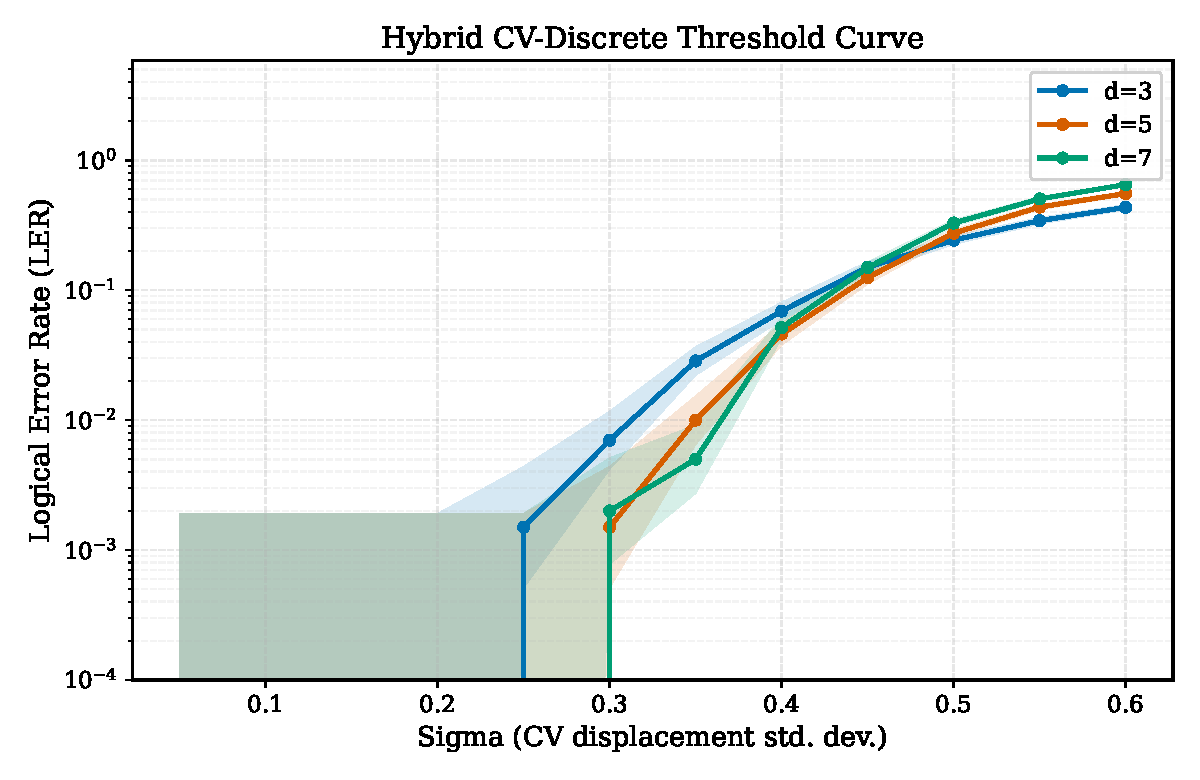
\includegraphics[keepaspectratio,alt={Representative LiDMaS+ output: logical error rate versus CV noise scale for distances d=3,5,7 in hybrid mode. This figure is generated by the reproducible examples/hybrid\_threshold workflow.}]{paper/figures/hybrid_threshold.pdf}}
\caption{Representative LiDMaS+ output: logical error rate versus CV
noise scale for distances d=3,5,7 in hybrid mode. This figure is
generated by the reproducible
\protect\texttt{examples/hybrid\_threshold} workflow.}
\end{figure}

\section{Statement of need}\label{statement-of-need}

Reliable threshold estimation in quantum error correction requires two
things: physically meaningful error models and reproducible, inspectable
simulation pipelines. In many projects, these are split across scripts,
ad hoc post-processing, and multiple codebases, which makes verification
and peer review difficult. LiDMaS+ addresses this gap by combining noise
generation, decoding, statistical aggregation, and plotting-ready
outputs into one auditable workflow.

The target audience includes researchers developing or benchmarking QEC
decoders, students reproducing threshold studies, and teams preparing
software-centered research artifacts (e.g., JOSS and arXiv
reproducibility appendices). The package is designed to support
deterministic reruns (fixed seeds), explicit confidence reporting, and
scriptable experiment definitions suitable for CI and review.

Unlike workflows that couple noise simulation and decoding through
external scripting pipelines, LiDMaS+ integrates noise generation,
pluggable decoding, statistical aggregation, and exportable artifacts
into a single auditable executable, reducing hidden variability in
threshold experiments.

\section{State of the field}\label{state-of-the-field}

Surface-code simulation and decoder benchmarking are active areas with
strong existing tools such as the high-performance stabilizer simulator
Stim \citep{stim2021} and matching-based decoding libraries such as
PyMatching \citep{pymatching2021}, as well as Union-Find decoders
\citep{unionfind2017}. LiDMaS+ is not intended to replace these mature
ecosystem components; rather, it provides an integrated experiment
harness centered on threshold workflows where users can switch between
Pauli and hybrid CV-discrete noise modes using one consistent interface.

In photonic and CV-oriented fault-tolerance research, related work from
Xanadu has explored static linear-optics fault tolerance and code
constructions relevant to overhead reduction
\citep{tzitrin2021static, sabo2024weightreduced}.

The distinguishing contribution is the unified end-to-end path from CV
Gaussian sampling to GKP-style digitization to surface-code decoding and
statistical reporting, alongside a modular decoder interface and
reproducible example suite. This ``single workflow, multiple noise
assumptions'' design simplifies controlled comparisons and reduces
hidden analysis variability between runs. Relative to the earlier LiDMaS
framing \citep{wayo2026lidmas}, LiDMaS+ emphasizes reproducible
threshold pipelines, pluggable decoding backends, and standardized
artifact generation for publication workflows.

\section{Software design}\label{software-design}

LiDMaS+ follows a modular architecture with clear separation between (1)
lattice/code construction, (2) noise generation, (3) decoder plugins,
(4) threshold runner/statistical aggregation, and (5) examples/plotting
scripts.

Key design choices include:

\begin{itemize}
\tightlist
\item
  Decoder plugin abstraction: \texttt{mwpm}, \texttt{uf}, and
  \texttt{neural\_mwpm} share a common interface, enabling controlled
  decoder swaps without changing experiment logic.
\item
  Mode-separated sweep control: \texttt{pauli} sweeps over physical
  error rate \texttt{p}, while \texttt{hybrid} sweeps over CV
  displacement scale \texttt{sigma}; the CLI rejects mixed sweep
  definitions for clarity.
\item
  Reproducibility-first execution: deterministic seed mixing per trial,
  fixed smoke configuration, and scripted examples with centralized
  result directories.
\item
  Statistical output by default: logical error rate with Wilson
  intervals, plus per-point diagnostics (defect and correction-weight
  summaries).
\end{itemize}

Mathematically, the two noise modes are separated as follows. In Pauli
mode, each data qubit is sampled from a depolarizing channel, \[
\Pr(I)=1-p,\quad \Pr(X)=\Pr(Y)=\Pr(Z)=p/3.
\] In hybrid mode, for each qubit we draw continuous displacements \[
(\Delta q,\Delta p)\sim \mathcal{N}(0,\sigma^2)\times\mathcal{N}(0,\sigma^2),
\] then digitize them using the GKP lattice scale \(s=\sqrt{\pi}\): \[
n_q=\mathrm{round}(\Delta q/s),\quad n_p=\mathrm{round}(\Delta p/s),
\] \[
x_{\mathrm{flip}} = (|n_q|\bmod 2),\quad z_{\mathrm{flip}} = (|n_p|\bmod 2).
\] The logical error rate is estimated from Monte Carlo counts as \[
\hat{p}_L = N_{\mathrm{fail}}/N_{\mathrm{trials}},
\] with Wilson interval at confidence level \(1-\alpha\): \[
\hat{p}_{L,\pm}=
\frac{\hat{p}_L+\frac{z^2}{2N}\pm z\sqrt{\frac{\hat{p}_L(1-\hat{p}_L)}{N}+\frac{z^2}{4N^2}}}
{1+\frac{z^2}{N}},
\quad z=\Phi^{-1}(1-\alpha/2).
\] For hybrid threshold sweeps, a practical crossing estimator between
distances \(d_1,d_2\) is computed on the sampled grid by \[
\sigma_{\mathrm{cross}}(d_1,d_2)\approx
\arg\min_{\sigma\in\Sigma}\left|\hat{p}_L(d_1,\sigma)-\hat{p}_L(d_2,\sigma)\right|.
\]

These choices prioritize transparent experimental method over opaque
performance-only optimization, aligning with reproducibility and
reviewability requirements.

\section{Research impact statement}\label{research-impact-statement}

LiDMaS+ is structured to support immediate scholarly use in
threshold-method studies and reproducibility packages. The repository
includes curated examples for smoke validation, Pauli threshold
baselines, hybrid CV sweeps, decoder comparison, and scaling-analysis
workflows. This supports two immediate practical outcomes:

\begin{enumerate}
\def\labelenumi{\arabic{enumi}.}
\tightlist
\item
  Fast independent verification of simulation behavior through
  deterministic, minimal smoke runs.
\item
  Consistent generation of figures and CSV artifacts suitable for
  publication appendices and method replication.
\end{enumerate}

At the time of submission, the software impact is demonstrated through
released, versioned workflows and reproducible experiment scripts.
Future work includes broader benchmarking and external integrations.

\section{AI usage disclosure}\label{ai-usage-disclosure}

Generative AI assistance was used during software development support
and paper drafting. Tooling included large-language-model assistants for
code-edit proposals, refactoring suggestions, and copy-editing of
documentation text. Human authors made the architectural decisions,
manually reviewed all generated content, executed validation runs, and
verified that final claims, equations, and outputs match the released
software behaviour.

\section{Acknowledgements}\label{acknowledgements}

The authors acknowledge contributors, users, and reviewers who provided
feedback on decoding workflows, reproducibility scripts, and
documentation quality.

This work was not funded.

\renewcommand\refname{References}
\bibliography{paper.bib}

\end{document}
